%%
%% Template chap2.tex
%%

\chapter{Results}
\label{cha:results}

\section{Instrumenting Beagle}
\label{section:instr}

\subsection{Beagle Before Indexing}
\label{sec:preindexing}

We have stated several times throughout this report that the key area of improvement for \beagle
is in clause resolution. However we have yet to provide any evidence to that fact.
Here we provide some results from initial investigations (before Fingerprint Indexing
was implemented) used to identify the key areas of improvement for \beagle.

\subsection{Indexing Simplification and Matching}

Refer to results for instrumentation; showing what may be improved with indexing.


\section{Indexing Metrics}
\label{sec:metrics}
In order to instrument the final version of \beagle\ with term indexing
we will no longer use VisualVM. 

Instead we shall introduce timing calls throughout the program 

Also includes number of inferences and false positive counts.

\subsection{Problem Selection}
We will wish to compare many different versions of \beagle, making a full run of TPTP
exceedingly impractical given the available time and resources (\citeN{shulz12}
made use of the University of Miami \emph{Peagsus Cluster} to run his tests). Thus
we must select a subset of problems which we may perform our tests against.
In creating this test we must be \emph{fair} in the sense of not selecting
problems which favour indexing; but we also are not interested in problems where
indexing is not used.

\subsection{Speed}

\subsection{False Positives}
Explain this metric and how it impacts performance.

Not as good results due to extreme other conditions on inference rules.
refer to differences in background rules. Also matching subterms!
Cheap throwaway FPs are not a concern.
totally useless even. Comment on change in how they are measured.

We observe many, even after a myriad of optimisations. Notice
that this is due to the structure of beagle; many retrieved terms
are cheaply thrown out due to other conditions (such as being a parent
term, being ordered, etc.) and do not significantly impact performance.

Refer to email from Stephan. compare false positive results

It is possible to na\"{\i}vley boost false positives to 0 by indexing a
huge number of positions; but this would not yield any speed improvement. Balancing false positive count with fingerprint
length is key.

\subsection{Runtime Per Inference}

\section{Comparing Versions of \Beagle}
\label{sec:indexresults}

In this section we present results and analysis for performance against the TPTP
problems and metrics discussed in Section \ref{sec:metrics} above. We discuss
three different versions of the prover:
\begin{itemize}
\item \textbf{Unmodified:} \beagle\ at the commencement of this project; without
any use of Fingerprint Indexing.
\item \textbf{Standard:} \beagle\ with the standard implementation of Fingerprint
Indexing; lacking our tailored optimisations from Section \ref{sec:tailored}. Both
Superposition and Simplification are indexed.
\item \textbf{Enhanced:} The full implementation described in this report; including
tailored optimisations.
\end{itemize}
Note that the performance of the two indexed versions can vary depending on what
positions we sample in order to generate Term Fingerprints. For the purpose of this
test we will have both the standard and the enhanced versions sample the following
positions:
  \[\epsilon,\  1,\  2,\  3,\  1.1,\  1.2\]
This set is named FP6M by \citeN{shulz12}, and it achieved the best performance in
his paper.

\begin{table}[H]\begin{center}
  \caption{Totalled inference counts and indexing statistics for various versions of \beagle.}
\begin{tabular}{| l || r | r | r || r | r | r |}  \cline{2-7}
\multicolumn{1}{ c }{} & \multicolumn{3}{ |c|| }{\textbf{Inference Counts}} & \multicolumn{3}{ c| }{\textbf{Indexing Results}} \\ \cline{1-7}
Version&Sup&Demod&NegUnit&TotalFound&SupFP&SimpFP\\  \cline{1-7}
\textbf{Unmodified \footnotemark[1]}&414216&29097&1826&0&0&0\\
\textbf{Standard}&162881&41414&2452&61884768&15525&39778148\\
\textbf{Enhanced}&146861&35326&1960&58119897&17641&39916687\\  \hline
\end{tabular}\end{center}\end{table}

\begin{table}[H]\begin{center}
  \caption{Totalled timing results for various versions of \beagle.}
\begin{tabular}{| l || r | r | r | r | r | r |}  \cline{2-7}
\multicolumn{1}{ c }{} & \multicolumn{6}{| c| }{\textbf{Time Spent (seconds)}} \\ \cline{1-7}
Version&Indexing&Retrieving&Sup&Demod&NegUnit&Total\\  \cline{1-7}
\textbf{Unmodified \footnotemark[1]}&0&0&730.44&9.44&31.99&5623.21\\
\textbf{Standard}&28.4&38.73&254.17&41.66&3.18&381.36\\
\textbf{Enhanced}&18.74&17.58&168.79&30.56&2.12&259.02\\ \hline
\end{tabular}\end{center}\end{table}

\footnotetext[1]{This version failed to solve two problems within 8 hours (28800 seconds).
These results are not included in the totals. See verbose table of results (Section \ref{sec:unres})}

\subsection{Performance Against Indexing Metrics}

\subsubsection{Total Time}
Looking only at the final total runtime for the three programs it would appear as
though using indexing has resulted in an improvement of over 95\% from 5623 seconds
to 259. In addition to this, the unmodified version also failed to solve two
DAT problems entirely when given 8 hours (28800 seconds) to solve each one.
Unfortunately however this improvement cannot be entirely attributed to
our implementation of Fingerprint Indexing; and as mentioned in Section \ref{sec:metrics}
we must be careful to consider all factors. In particular, notice that the unmodified
version performs 414216 superposition inferences, nearly three times that of our
final enhanced implementation. This sort of discrepancy is not entirely unexpected,
and is essentially a fluke introduced by changing the order inferences are performed.
With this in mind the 95\% improvement is no longer relevant; and we must look into alternative
measures of performance.

Notice however that the standard version of beagle only performs about 10\% more
superposition inferences than the enhanced version; making these two versions much more comparable
on total time. Between these two versions we observe a total run time improvement
of 122 seconds, or about 2.5 seconds per problem. Of particular interest in comparing
these two versions is the difference between time spent retrieving from the index.
We notice that the enhanced version spends about 50\% less time performing retrievals;
even though it uses a far more complicated comparison table function (compare Listing
\ref{lst:unitable} for the standard version to Listing \ref{lst:extuni} for enhanced).
The speed up must then come from a reduced need to traverse the Fingerprint Index
due to less matching fingerprints; implying that our tailored improvements are greatly
improving the efficiency of Fingerprint Indexing.


\subsubsection{False Positives}
When we examine the count for false positives it does not immediately reflect our
above finding that the enhanced version has improved the efficiency of indexing.
In fact we observe over 10\% \emph{more} superposition false positives in the enhanced
version (and about 0.5\% more simplification false positives). This seems to contradict
our raw timing results; but the contradiction may be resolved by considering all factors involved.

An indexing false positive obviously results in some unnecessary computation as we
have attempted unification and failed. However, even after unification succeeds we may
still fail to perform superposition due to other restrictions of the inference rule.
In particular there are four Literal and Term ordering restrictions which must
be checked \emph{after} verifying unification, as they require the substitution
used (see Section \ref{sec:calc}). This means that even when a term
is not counted as a false positive for unification it may still cause the same
amount of unnecessary computation.

Thus we must consider the TotalFound column, which counts the total number of terms
retrieved from the index; regardless of whether or not they result in unification or an inference.
In this column we observe a superb improvement in the enhanced version
of \beagle, with it retrieving almost four million fewer terms than the standard index.
This difference is direct evidence of tailored enhancements reducing the amount of index traversal necessary;
and unlike the false positive count we can be sure that each term not retrieved
is saving us some amount of computation. This explains how we can have 2116 more
false positives and still see a significant increase in performance; but we still
have not seen how these extra false positives could have occurred.

The difference is small enough that we can again consider it a fluke arising from
the variation in inference order. This is very unsatisfying however since our
improved unification table from Section \ref{sec:extunif} should result specifically
in fewer false positives; not just fewer terms retrieved from the index. 
Recall that the extended table works by considering the placement of terms
in the hierarchy (whether they are foreground or background). Thus the improvement will only
be relevant when there are a reasonable percentage of background terms; such as in
arithmetic problems.
When examining only the set of ten ARI problems 
(see the verbatim result tables in Appendix \ref{app:app1}) we observe
that the enhanced version is superior by all measures of performance.
In fact we observe a total of \emph{zero}
superposition false positives versus 124 for the standard version. This result shows the true worth of our
improved unification table, as it is not necessarily relevant in the case of DAT, PUZ
and GRP problems. Our additional tailored improvements from Section \ref{sec:otherimp}
are still relevant for these problems and produce the significant improvement
seen in total terms retrieved.



\subsubsection{Time Per Inference}

 \begin{table}[H]\begin{center}
  \caption{Total time spent per inference for various versions of \beagle.}
\begin{tabular}{| l || r | r | r |}  \hline
Version&Superposition&Demodulation&NegUnit Simplification\\  \hline
\textbf{Unmodified}&1.7ms & 0.3ms & 17.5ms  \\
\textbf{Standard}  &1.5ms & 1.0ms & 1.3ms  \\
\textbf{Enhanced}  &1.1ms & 0.8ms & 1.0ms  \\\hline
\end{tabular}\end{center}\end{table}  


\subsection{Results for Small Problems}

\begin{figure}[h]
  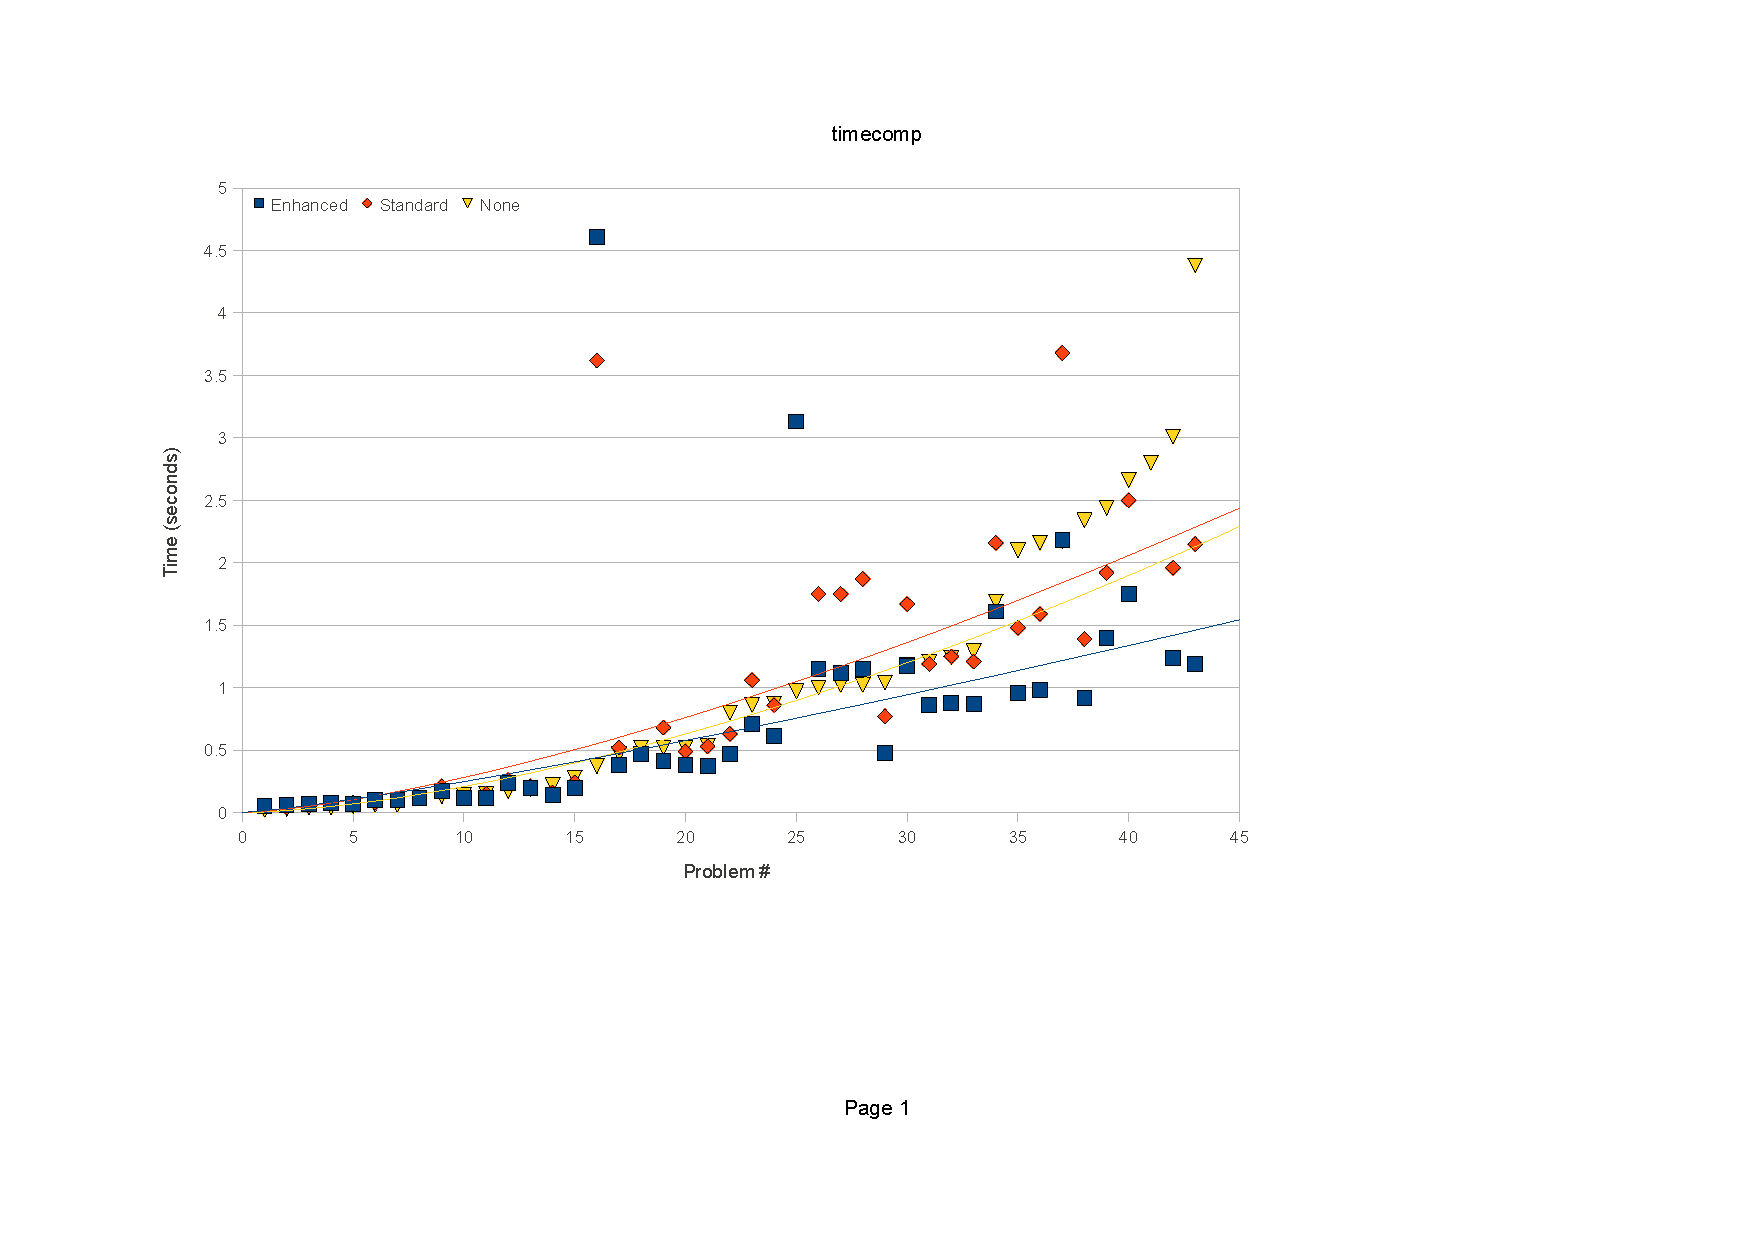
\includegraphics[trim=2.45cm 5cm 8cm 3cm,clip,width=\textwidth]{resources/suptimetrends}
  \caption{Superposition time comparison for three versions of \beagle\ for small problems
  (under 5 seconds of superposition)}
\end{figure}

\subsection{Results for Large Problems}

\section{Comparing Various Fingerprint Sampling Positions}

  \begin{itemize}
  \item FP3W: Samples 3 positions to a maximum depth of 2. While this set creates
  tiny Fingerprints it was still able to achieve good results due to the relative simplicity
  of retrieving from the index. \cite{shulz12}
  \[\epsilon,\  1,\  2\]
  \item FP4M: Samples 4 positions to a maximum depth of 3.
  \[\epsilon,\  1,\  2,\  1.1\]
  \item FP6M: Samples 6 positions to a maximum depth of 3. This set produced the
  best performance in the tests by \citeN{shulz12}.
  \[\epsilon,\  1,\  2,\  3,\  1.1,\  1.2\]
  \item FP7: Samples 7 positions to a maximum depth of 3.
  \[\epsilon,\  1,\  2,\  1.1,\  1.2,\  2.1,\  2.2\]
  \item FP8X2: Samples 16 positions. This is an example of excessively large Fingerprints
  which should result in a steep decrease in performance.
  \[\epsilon,\  1,\  2,\  3,\  4,\  1.1,\  1.2,\  1.3,\  2.1,\  2.2,\  2.3,\  3.1,\  3.2,\  3.3,\  1.1.1,\  2.1.1\]
  \end{itemize}


\begin{table}[H]\begin{center}
  \caption[]{Totalled inference counts and indexing statistics for various Fingerprint sampling sets.\footnotemark[1]}
\begin{tabular}{| l || r | r | r || r | r | r |}  \cline{2-7}
\multicolumn{1}{ c }{} & \multicolumn{3}{ |c|| }{\textbf{Inference Counts}} & \multicolumn{3}{ c| }{\textbf{Indexing Results}} \\ \cline{1-7}
Sample Set&Sup&Demod&NegUnit&TotalFound&SupFP&SimpFP\\  \cline{1-7}
\textbf{FP3W}&162218&42402&2472&13913606&69429&1815992\\
\textbf{FP4M}&147798&35709&1963&13469779&26847&1851515\\
\textbf{FP6M}&144505&35326&1959&12601762&16406&1694731\\
\textbf{FP7}&159055&41005&2440&13011130&21281&1596575\\
\textbf{FP8X2}&159385&40876&2438&12819184&11229&1602033\\ \hline 
\end{tabular}\end{center}\end{table}

\begin{table}[H]\begin{center}
  \caption[]{Totalled timing results for various Fingerprint sampling sets.\footnotemark[1]}
\begin{tabular}{| l || r | r | r | r | r | r |}  \cline{2-7}
\multicolumn{1}{ c }{} & \multicolumn{6}{| c| }{\textbf{Time Spent (seconds)}} \\ \cline{1-7}
Sample Set&Indexing&Retrieving&Sup&Demod&NegUnit&Total\\  \cline{1-7}
\textbf{FP3W}&11.52&14.02&170.37&9.26&1.78&237.75\\
\textbf{FP4M}&13.09&14.12&164.95&9.51&1.82&230.68\\
\textbf{FP6M}&16.82&16.5&159.93&10.78&2.11&229.59\\
\textbf{FP7}&19.98&18.74&170.83&12.37&2.37&249.22\\
\textbf{FP8X2}&45.56&32.59&181.43&21.45&4.06&294.8\\ \hline 
\end{tabular}\end{center}\end{table}

\footnotetext[1]{Excludes problem PUZ037-1.p}
%%% Local Variables: 
%%% mode: latex
%%% TeX-master: "thesis"
%%% End: 
